% ============================================================
%  Appendices
% ============================================================

\appendix
\addcontentsline{toc}{chapter}{Appendices}
\chapter*{Appendices}
\markboth{Appendices}{}

% ============================================================
\chapter{Hyperparameter Tuning Details}
\label{app:tuning}
% ============================================================

This appendix documents the search spaces explored during Bayesian hyperparameter optimisation with Optuna~\cite{optuna2019} and the best configurations obtained for each model family on the 6-month horizon.
All experiments use 60 TPE trials, GroupKFold($k{=}5$) cross-validation on the DEV partition ($n{=}1{,}113$), and PR-AUC (average precision) as the objective.

% ---------- Search spaces ----------
\section{Search Spaces}
\label{app:search_spaces}

Table~\ref{tab:search_spaces} lists the hyperparameter ranges explored for each of the seven model families.

\begin{table}[htbp]
\centering
\caption[Optuna hyperparameter search spaces]{Hyperparameter search spaces used in Optuna TPE optimisation.}
\label{tab:search_spaces}
\small
\begin{tabular}{l l l l}
\toprule
\textbf{Model} & \textbf{Hyperparameter} & \textbf{Range / Values} & \textbf{Scale} \\
\midrule
\multirow{3}{*}{KNN}
  & \texttt{n\_neighbors}      & $[3,\,51]$, step=2       & linear \\
  & \texttt{weights}           & \{uniform, distance\}    & categorical \\
  & \texttt{metric}            & \{euclidean, manhattan\}  & categorical \\
\midrule
\multirow{4}{*}{Decision Tree}
  & \texttt{max\_depth}        & $[2,\,20]$               & linear \\
  & \texttt{min\_samples\_split} & $[2,\,50]$             & linear \\
  & \texttt{min\_samples\_leaf}  & $[1,\,30]$             & linear \\
  & \texttt{criterion}         & \{gini, entropy\}        & categorical \\
\midrule
\multirow{5}{*}{Random Forest}
  & \texttt{n\_estimators}     & $[100,\,800]$, step=50   & linear \\
  & \texttt{max\_depth}        & $[3,\,20]$               & linear \\
  & \texttt{min\_samples\_split} & $[2,\,30]$             & linear \\
  & \texttt{min\_samples\_leaf}  & $[1,\,20]$             & linear \\
  & \texttt{max\_features}     & \{sqrt, log2\}           & categorical \\
\midrule
\multirow{3}{*}{SVM}
  & \texttt{C}                 & $[10^{-2},\,100]$        & log \\
  & \texttt{kernel}            & \{rbf, linear\}          & categorical \\
  & \texttt{gamma} (if rbf)    & $[10^{-4},\,1]$          & log \\
\midrule
\multirow{2}{*}{Logistic Reg.}
  & \texttt{C}                 & $[10^{-3},\,50]$         & log \\
  & \texttt{penalty}           & \{l1, l2\}               & categorical \\
\midrule
\multirow{9}{*}{LightGBM}
  & \texttt{n\_estimators}     & $[200,\,1200]$, step=50  & linear \\
  & \texttt{learning\_rate}    & $[0.01,\,0.20]$          & log \\
  & \texttt{num\_leaves}       & $[15,\,127]$             & linear \\
  & \texttt{max\_depth}        & $[-1,\,12]$              & linear \\
  & \texttt{min\_child\_samples} & $[5,\,50]$             & linear \\
  & \texttt{subsample}\textsuperscript{a} & $[0.6,\,1.0]$            & linear \\
  & \texttt{colsample\_bytree} & $[0.6,\,1.0]$            & linear \\
  & \texttt{reg\_lambda}       & $[10^{-3},\,10]$         & log \\
  & \texttt{reg\_alpha}        & $[10^{-6},\,1]$          & log \\
\midrule
\multirow{9}{*}{XGBoost}
  & \texttt{n\_estimators}     & $[200,\,1200]$, step=50  & linear \\
  & \texttt{learning\_rate}    & $[0.01,\,0.20]$          & log \\
  & \texttt{max\_depth}        & $[2,\,8]$                & linear \\
  & \texttt{min\_child\_weight}& $[1,\,20]$               & log \\
  & \texttt{subsample}         & $[0.6,\,1.0]$            & linear \\
  & \texttt{colsample\_bytree} & $[0.6,\,1.0]$            & linear \\
  & \texttt{gamma}             & $[0,\,5]$                & linear \\
  & \texttt{reg\_lambda}       & $[10^{-3},\,10]$         & log \\
  & \texttt{reg\_alpha}        & $[10^{-6},\,1]$          & log \\
\bottomrule
\end{tabular}
\par\smallskip
{\scriptsize \textsuperscript{a}Sampled in the recorded LightGBM runs but inactive because \texttt{subsample\_freq} remained at its default value of 0.}
\end{table}


% ---------- Best hyperparameters ----------
\section{Best Hyperparameters (6-Month Horizon)}
\label{app:best_params}

Tables~\ref{tab:best_simple}--\ref{tab:best_boosting} report the best configuration found for each model on the 6-month DEV set.
For models evaluated in both balanced and unbalanced modes, the configuration with the higher PR-AUC is indicated in bold.
The LightGBM \texttt{subsample} values are retained to reproduce the stored trial records, but were inactive because \texttt{subsample\_freq=0}.

\begin{table}[htbp]
\centering
\caption[Best hyperparameters: simple models]{Best hyperparameters --- simple models (6-month horizon).}
\label{tab:best_simple}
\small
\begin{tabular}{l l c c}
\toprule
\textbf{Model} & \textbf{Hyperparameter} & \textbf{Balanced} & \textbf{Unbalanced} \\
\midrule
\multirow{4}{*}{KNN}
  & \texttt{n\_neighbors}      & ---   & 51 \\
  & \texttt{weights}           & ---   & distance \\
  & \texttt{metric}            & ---   & euclidean \\
  & PR-AUC                     & ---   & 0.387 \\
\midrule
\multirow{5}{*}{Decision Tree}
  & \texttt{criterion}         & entropy & entropy \\
  & \texttt{max\_depth}        & 7       & 11 \\
  & \texttt{min\_samples\_split} & 19    & 42 \\
  & \texttt{min\_samples\_leaf}  & 12    & 5 \\
  & PR-AUC                     & \textbf{0.404} & 0.388 \\
\midrule
\multirow{6}{*}{Random Forest}
  & \texttt{n\_estimators}     & 750   & 200 \\
  & \texttt{max\_depth}        & 4     & 9 \\
  & \texttt{max\_features}     & sqrt  & sqrt \\
  & \texttt{min\_samples\_split} & 8   & 24 \\
  & \texttt{min\_samples\_leaf}  & 20  & 12 \\
  & PR-AUC                     & 0.425 & \textbf{0.431} \\
\midrule
\multirow{4}{*}{SVM}
  & \texttt{kernel}            & rbf     & rbf \\
  & \texttt{C}                 & 38.84   & 69.93 \\
  & \texttt{gamma}             & 0.00174 & 0.00313 \\
  & PR-AUC                     & \textbf{0.426} & 0.389 \\
\midrule
\multirow{3}{*}{Logistic Reg.}
  & \texttt{penalty}           & l1    & l1 \\
  & \texttt{C}                 & 0.070 & 0.068 \\
  & PR-AUC                     & \textbf{0.407} & 0.401 \\
\bottomrule
\end{tabular}
\end{table}


\begin{table}[htbp]
\centering
\caption[Best hyperparameters: gradient boosting models]{Best hyperparameters --- gradient boosting models (6-month horizon).}
\label{tab:best_boosting}
\small
\begin{tabular}{l l c c}
\toprule
\textbf{Model} & \textbf{Hyperparameter} & \textbf{Balanced} & \textbf{Unbalanced} \\
\midrule
\multirow{10}{*}{LightGBM}
  & \texttt{n\_estimators}       & 700     & 200 \\
  & \texttt{learning\_rate}      & 0.0101  & 0.0160 \\
  & \texttt{num\_leaves}         & 117     & 127 \\
  & \texttt{max\_depth}          & 2       & 3 \\
  & \texttt{min\_child\_samples} & 44      & 30 \\
  & \texttt{subsample}           & 0.700   & 0.761 \\
  & \texttt{colsample\_bytree}   & 0.822   & 0.697 \\
  & \texttt{reg\_lambda}         & 0.761   & 0.097 \\
  & \texttt{reg\_alpha}          & $2.2 \times 10^{-6}$ & $9.6 \times 10^{-5}$ \\
  & PR-AUC                       & \textbf{0.418} & 0.415 \\
\midrule
\multirow{10}{*}{XGBoost}
  & \texttt{n\_estimators}       & 450     & 500 \\
  & \texttt{learning\_rate}      & 0.0153  & 0.0204 \\
  & \texttt{max\_depth}          & 6       & 8 \\
  & \texttt{min\_child\_weight}  & 7.922   & 1.013 \\
  & \texttt{subsample}           & 0.624   & 0.757 \\
  & \texttt{colsample\_bytree}   & 0.625   & 0.779 \\
  & \texttt{gamma}               & 4.755   & 3.674 \\
  & \texttt{reg\_lambda}         & 0.219   & 4.250 \\
  & \texttt{reg\_alpha}          & $4.9 \times 10^{-5}$ & $2.6 \times 10^{-6}$ \\
  & PR-AUC                       & 0.424   & \textbf{0.434} \\
\bottomrule
\end{tabular}
\end{table}


% ============================================================
\chapter{Feature Ablation Study}
\label{app:ablation}
% ============================================================

This appendix presents the cumulative feature-block ablation experiment.
Starting from a baseline of 15 demographic and ALSFRS-R features, successive blocks of clinical variables are added to assess their marginal contribution to model performance.

\begin{table}[htbp]
\centering
\caption[Feature block ablation PR-AUC, DEV set]{Feature block ablation (6-month, DEV set). PR-AUC with Optuna-tuned hyperparameters. Blocks are cumulative: each row adds new features to the previous.}
\label{tab:app_ablation}
\small
\begin{tabular}{lccccc}
\toprule
Block & $n_\text{features}$ & XGB\textsubscript{unb} & RF\textsubscript{unb} & LGBM\textsubscript{bal} & LR\textsubscript{bal} \\
\midrule
A: Baseline              & 15 & 0.420 & 0.409 & 0.434 & 0.395 \\
B: A + Vitals             & 27 & 0.420 & 0.408 & 0.420 & 0.405 \\
C: A + FVC                & 18 & 0.430 & 0.434 & 0.432 & 0.400 \\
D: A + Vitals + FVC       & 30 & 0.432 & 0.418 & 0.424 & 0.406 \\
E: D + Treatment          & 33 & 0.423 & 0.417 & 0.425 & 0.407 \\
F: Full v2                & 35 & 0.434 & 0.431 & 0.418 & 0.407 \\
\bottomrule
\end{tabular}
\end{table}

The ablation results show that FVC-derived features (block~C) provide the most consistent individual gains across models, consistent with FVC's established role as a key prognostic marker in ALS.
The full v2 feature set (block~F, 35~features) maximises XGBoost performance at 0.434 PR-AUC, the best overall configuration selected for final training.

\begin{figure}[htbp]
  \centering
  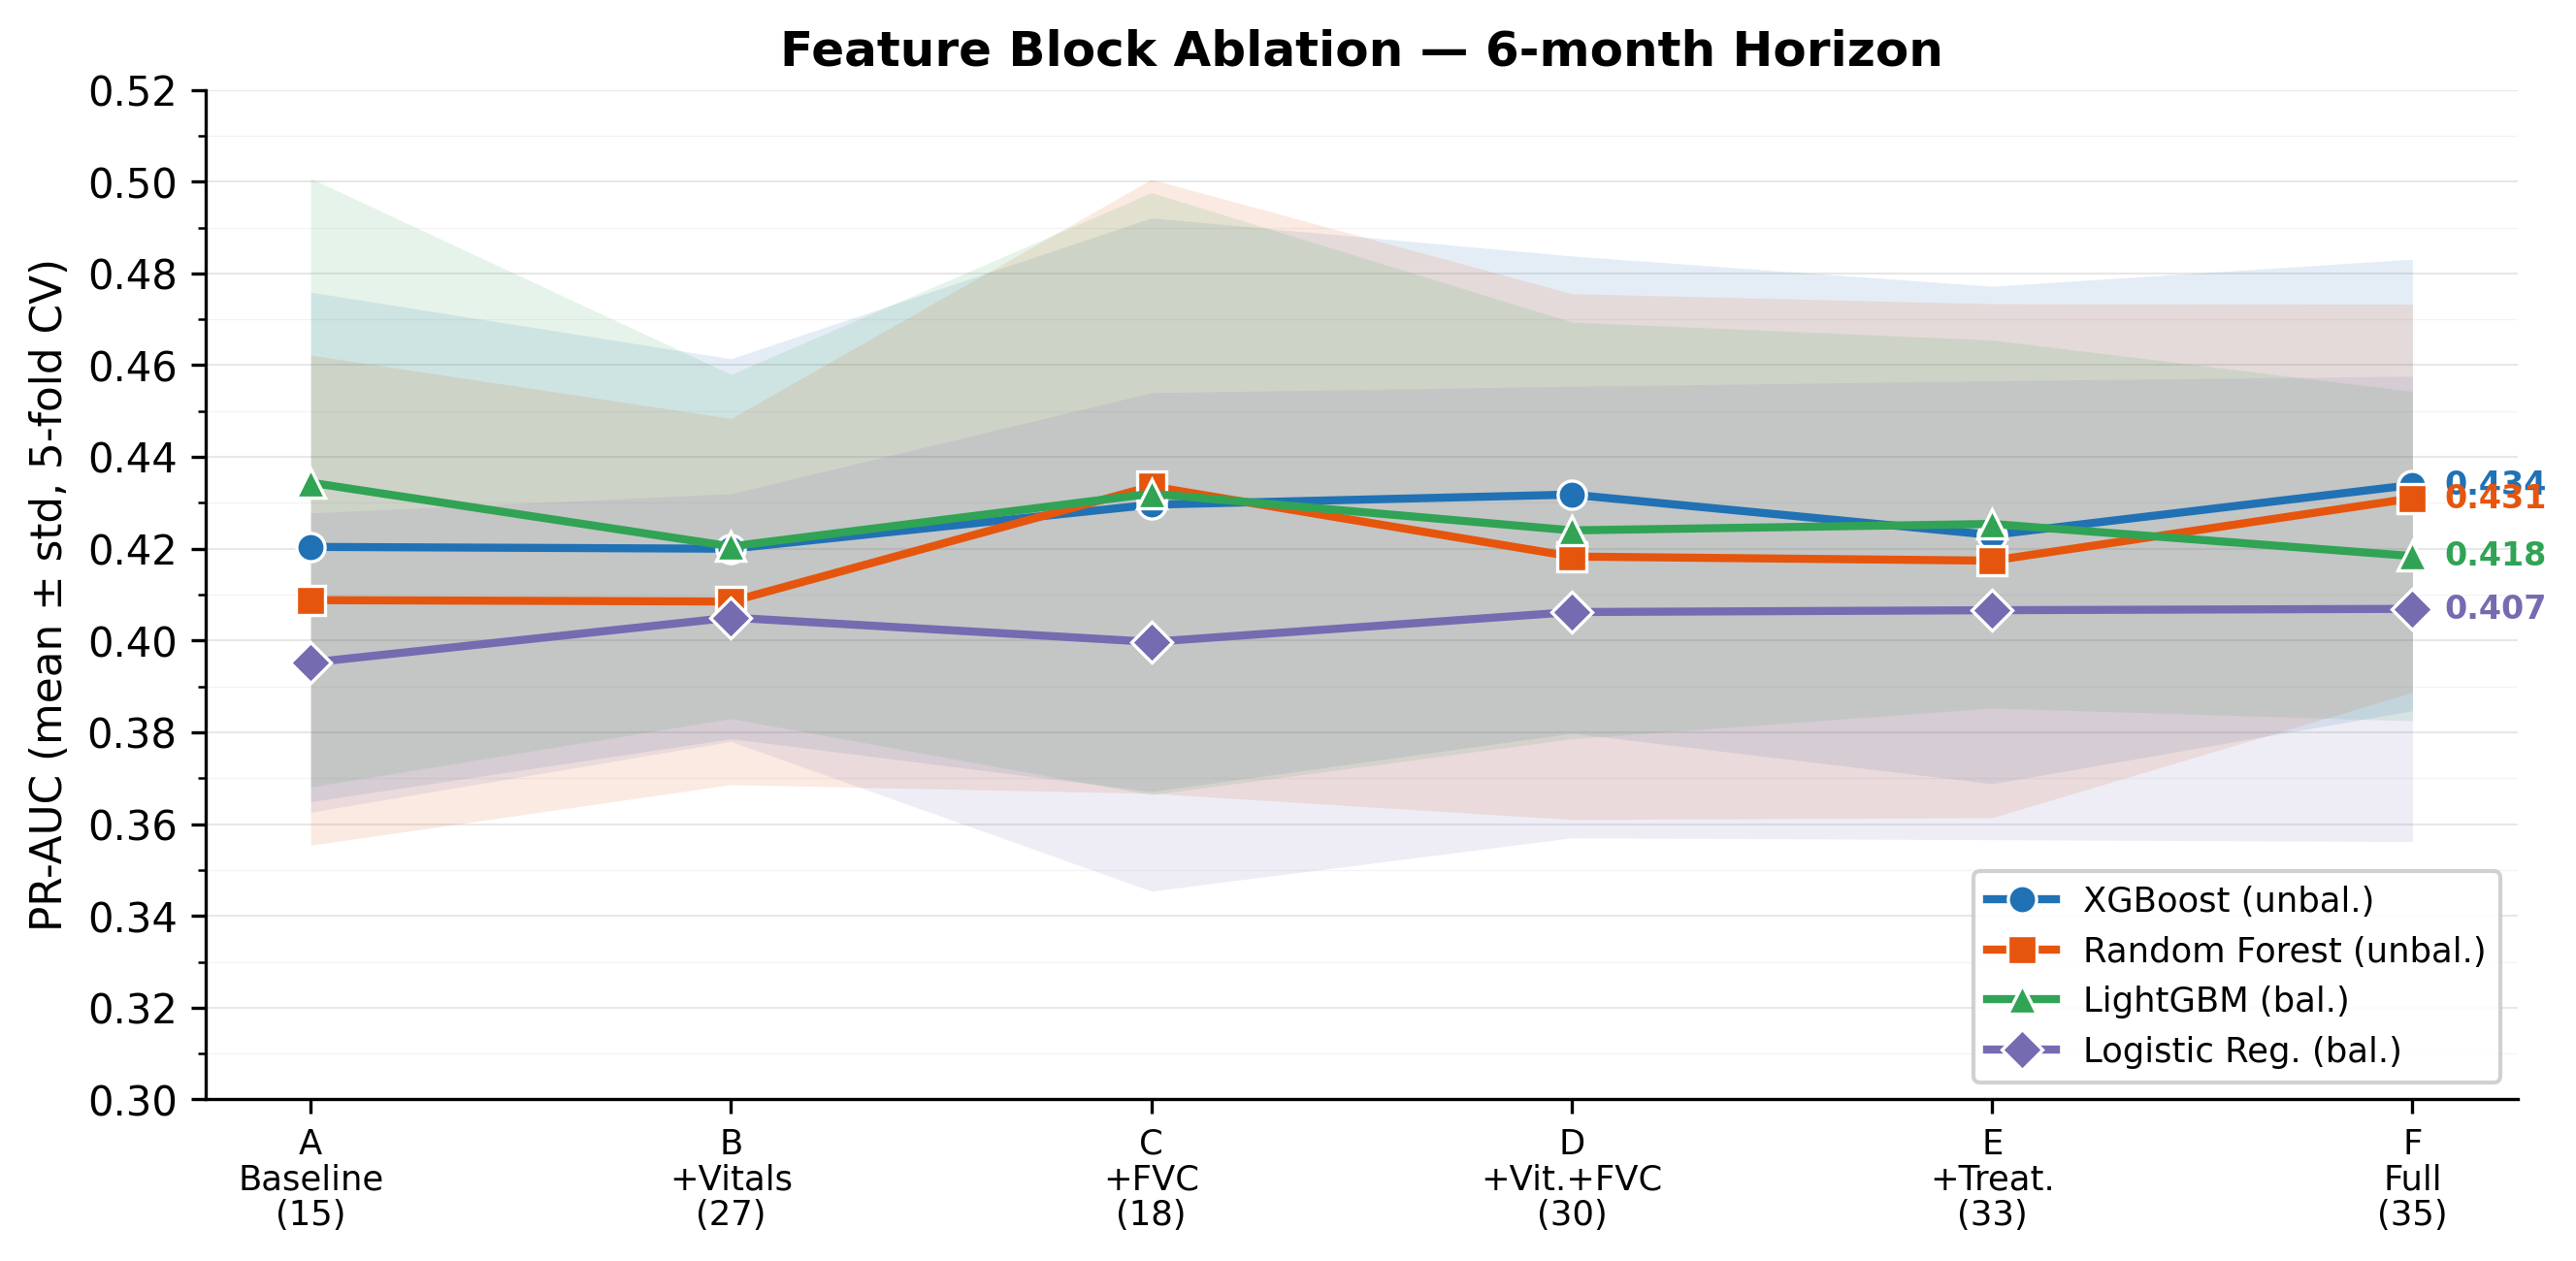
\includegraphics[width=0.85\linewidth]{./images/figures/step5v2_ablation_prauc.png}
  \caption[PR-AUC across cumulative feature blocks]{PR-AUC progression across cumulative feature blocks for four model families. FVC features (block~C) yield the largest marginal improvement.}
  \label{fig:app_ablation}
\end{figure}


% ============================================================
\chapter{Holdout Evaluation and Statistical Tests}
\label{app:holdout}
% ============================================================

This appendix reports the full held-out test set evaluation and the statistical comparison of the seven tuned model configurations.

% ---------- Test metrics ----------
\section{Test Set Performance}
\label{app:test_metrics}

Table~\ref{tab:app_test_metrics} presents the performance of all seven models on the held-out TEST partition ($n{=}279$, 20\% of the 6-month cohort), which was not used during hyperparameter tuning or model selection.

\begin{table}[htbp]
\centering
\caption[TEST set metrics, all 7 models (appendix)]{Held-out TEST set metrics (6-month horizon, $n{=}279$). PR-AUC and ROC-AUC are threshold-free; F$_1$ and F$_2$ use default $t{=}0.50$; Brier score measures calibration (lower is better).}
\label{tab:app_test_metrics}
\small
\begin{tabular}{l c c c c c c}
\toprule
Model & Mode & PR-AUC & ROC-AUC & F$_1$ & F$_2$ & Brier \\
\midrule
  XGBoost          & unbalanced & 0.456 & 0.660 & 0.085 & 0.058 & 0.1971 \\
  RandomForest     & unbalanced & \textbf{0.459} & 0.664 & 0.000 & 0.000 & 0.1986 \\
  SVM              & balanced   & 0.447 & 0.675 & 0.000 & 0.000 & 0.1977 \\
  LightGBM         & balanced   & 0.429 & 0.637 & 0.422 & 0.440 & 0.2241 \\
  LogisticRegression & balanced & 0.421 & 0.671 & 0.484 & 0.520 & 0.2307 \\
  DecisionTree     & balanced   & 0.373 & 0.569 & 0.417 & 0.417 & 0.2695 \\
  KNeighbors       & unbalanced & 0.393 & 0.583 & 0.046 & 0.029 & 0.2062 \\
\bottomrule
\end{tabular}
\end{table}


% ---------- Diagnostic curves ----------
\section{Diagnostic Curves}
\label{app:curves}

\begin{figure}[htbp]
  \centering
  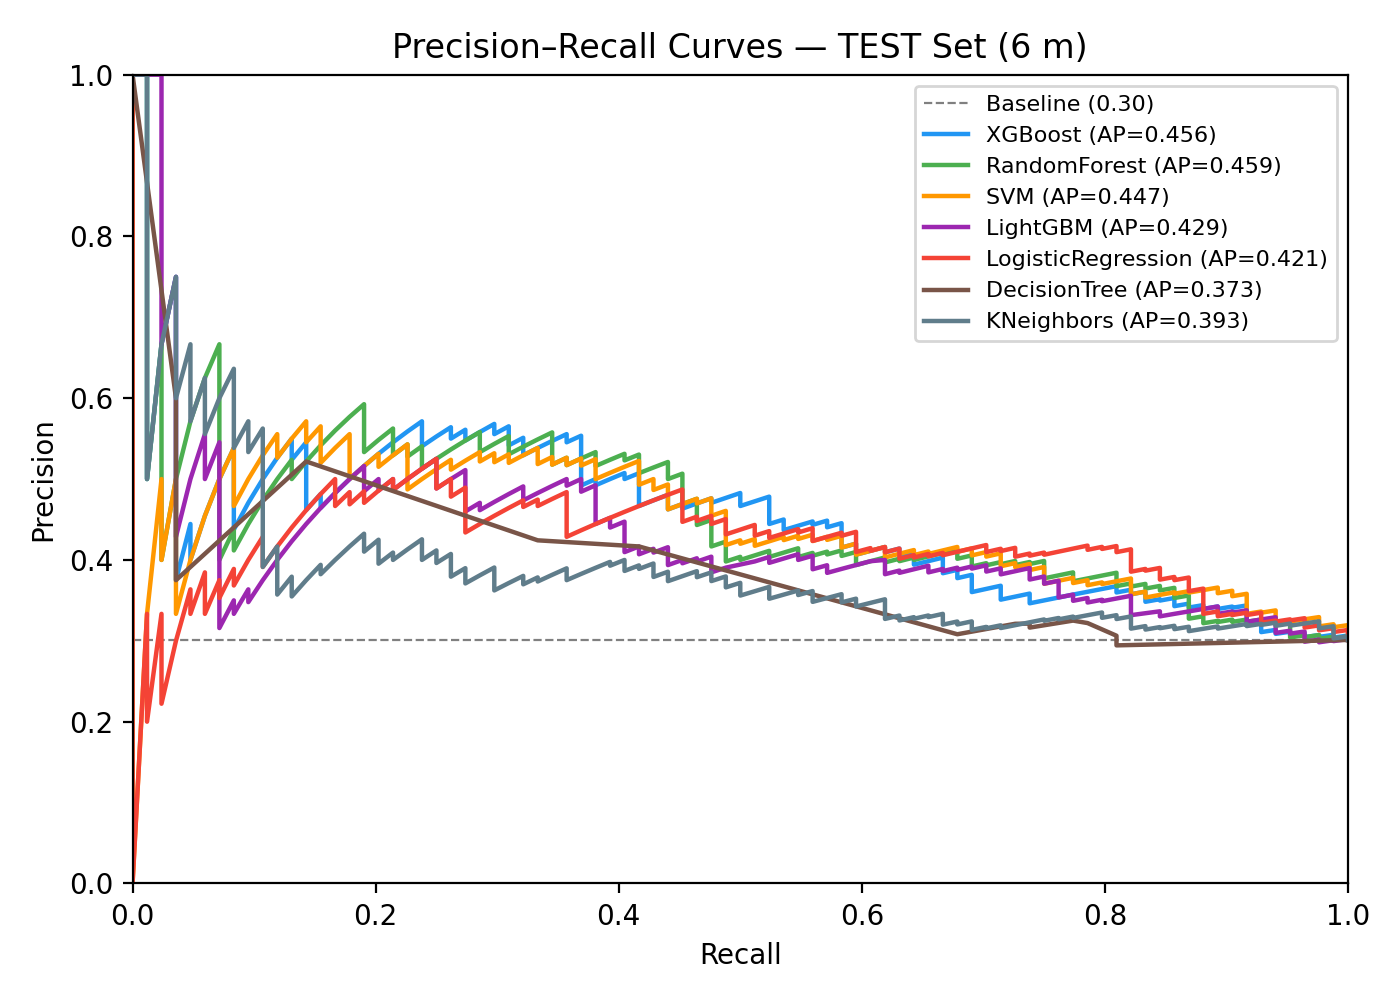
\includegraphics[width=0.85\linewidth]{./images/figures/step6_pr_curves.png}
  \caption[Precision--Recall curves, all 7 models]{Precision--Recall curves on the held-out TEST set for all seven models.}
  \label{fig:app_pr}
\end{figure}

\begin{figure}[htbp]
  \centering
  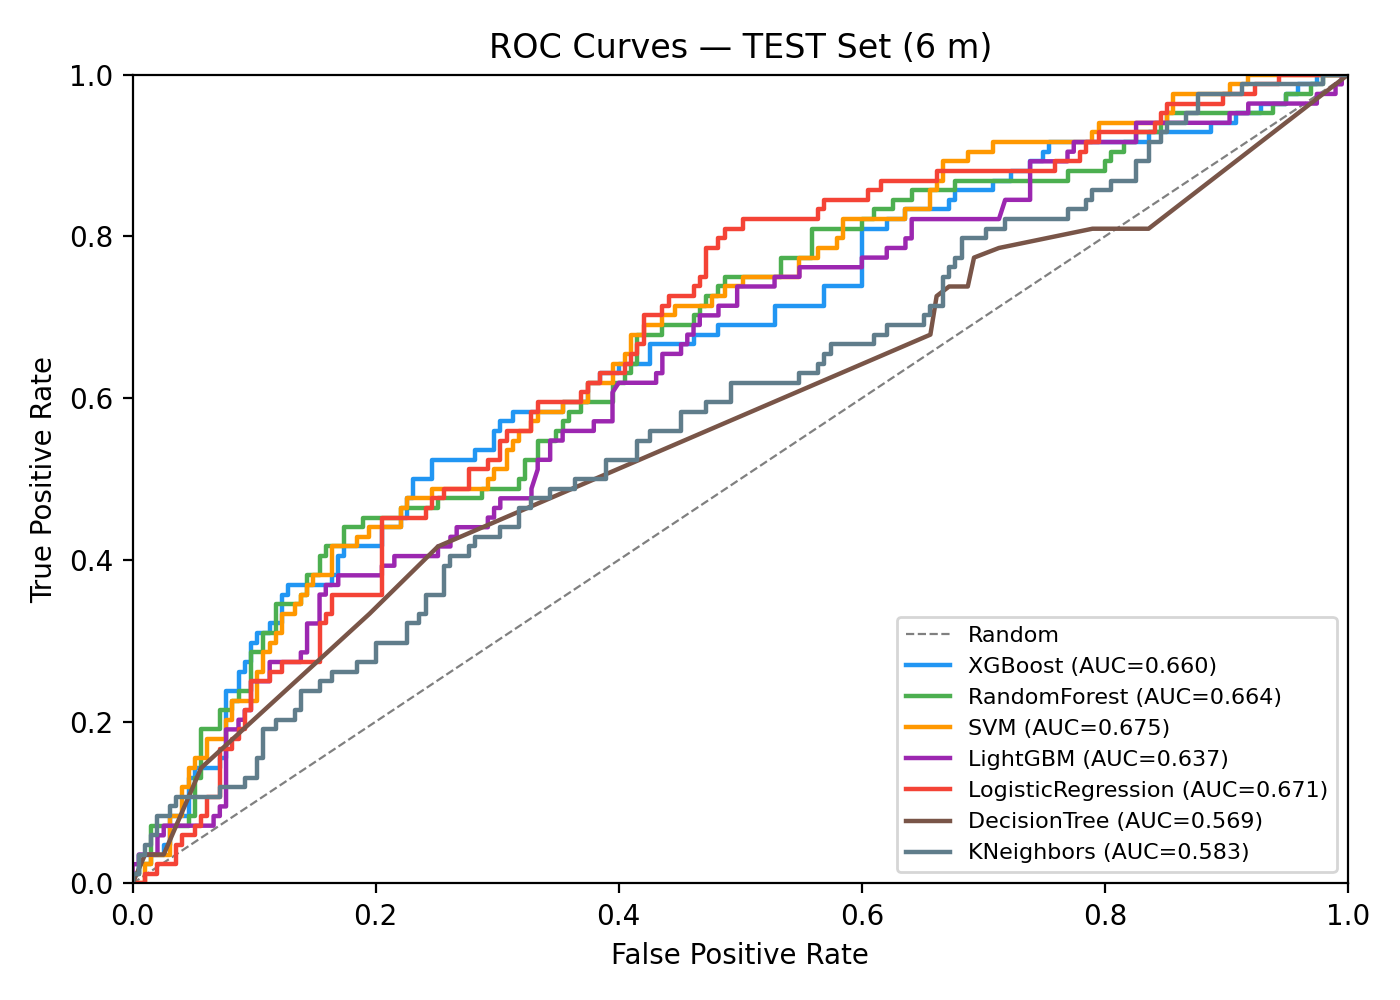
\includegraphics[width=0.85\linewidth]{./images/figures/step6_roc_curves.png}
  \caption[ROC curves, all 7 models]{ROC curves on the held-out TEST set.}
  \label{fig:app_roc}
\end{figure}

\begin{figure}[htbp]
  \centering
  
\includegraphics[width=0.85\linewidth]{./images/figures/step6_calibration.png}
  \caption[Calibration plots, all 7 models]{Calibration plots (reliability diagrams) for all seven models on the TEST set.}
  \label{fig:app_calibration}
\end{figure}

\begin{figure}[htbp]
  \centering
  
\includegraphics[width=0.85\linewidth]{./images/figures/step6_confusion_matrix.png}
  \caption[Confusion matrices at default threshold, all models]{Confusion matrices at the default threshold ($t{=}0.50$) on the TEST set.}
  \label{fig:app_cm}
\end{figure}


% ---------- Statistical comparison ----------
\section{Statistical Comparison}
\label{app:stats}

The Friedman test was the primary comparison of the per-fold PR-AUC ranks from 5-fold GroupKFold on the DEV set. As the omnibus test did not reject its null hypothesis, the pairwise Wilcoxon signed-rank tests below are included for descriptive completeness and are not treated as confirmatory post-hoc tests.

\begin{table}[htbp]
  \centering
  \caption[Exploratory pairwise Wilcoxon comparisons]{Exploratory pairwise Wilcoxon signed-rank comparisons with Bonferroni correction (Friedman $\chi^2_F(6) = 12.43$, $p = 0.0531$).}
  \label{tab:app_pairwise}
  \small
  \begin{tabular}{llccc}
    \toprule
    Model A & Model B & Statistic & $p_\text{raw}$ & $p_\text{Bonf.}$ \\
    \midrule
    XGB  & RF   & 6.0 & 0.8125 & 1.0000 \\
    XGB  & SVM  & 4.0 & 0.4375 & 1.0000 \\
    XGB  & LGBM & 2.0 & 0.1875 & 1.0000 \\
    XGB  & LR   & 0.0 & 0.0625 & 1.0000 \\
    XGB  & DT   & 0.0 & 0.0625 & 1.0000 \\
    XGB  & KNN  & 1.0 & 0.1250 & 1.0000 \\
    RF   & SVM  & 7.0 & 1.0000 & 1.0000 \\
    RF   & LGBM & 3.0 & 0.3125 & 1.0000 \\
    RF   & LR   & 1.0 & 0.1250 & 1.0000 \\
    RF   & DT   & 1.0 & 0.1250 & 1.0000 \\
    RF   & KNN  & 0.0 & 0.0625 & 1.0000 \\
    SVM  & LGBM & 4.0 & 0.4375 & 1.0000 \\
    SVM  & LR   & 1.0 & 0.1250 & 1.0000 \\
    SVM  & DT   & 1.0 & 0.1250 & 1.0000 \\
    SVM  & KNN  & 1.0 & 0.1250 & 1.0000 \\
    LGBM & LR   & 4.0 & 0.4375 & 1.0000 \\
    LGBM & DT   & 3.0 & 0.3125 & 1.0000 \\
    LGBM & KNN  & 3.0 & 0.3125 & 1.0000 \\
    LR   & DT   & 5.0 & 0.6250 & 1.0000 \\
    LR   & KNN  & 5.0 & 0.6250 & 1.0000 \\
    DT   & KNN  & 6.0 & 0.8125 & 1.0000 \\
    \bottomrule
  \end{tabular}
\end{table}

The Friedman test yields $\chi^2_F(6)=12.43$ ($p=0.053$; Kendall's $W=0.414$), so the null hypothesis of equal rank distributions is not rejected at $\alpha=0.05$. All 21 exploratory pairwise comparisons have $p_\text{Bonf.}=1.000$. With only five pairs, the minimum exact two-sided Wilcoxon $p$-value is 0.0625, making this outcome unavoidable after correction. The table therefore provides no evidence of pairwise differences, but it also cannot establish that the models are equivalent.
